\documentclass[conference]{IEEEtran}
\IEEEoverridecommandlockouts

\usepackage{amsmath,amssymb,amsfonts}
\usepackage{graphicx}
\usepackage{textcomp}
\usepackage{xcolor}
\usepackage{booktabs}
\usepackage{array}
\usepackage{url}
\usepackage{microtype}
\usepackage{tikz}
\usetikzlibrary{shapes.geometric, arrows.meta, positioning, fit, backgrounds}

% Make all monospace/code text slightly smaller than body text
\let\oldtexttt\texttt
\renewcommand{\texttt}[1]{{\small\oldtexttt{#1}}}

\begin{document}

\title{Weather-Integrated Crop Health Monitoring:\\
Deliverable 3 --- Refinements, Extended Evaluation,\\
and Responsible AI Reflection}

\author{
  \IEEEauthorblockN{Khang Phan}
  \IEEEauthorblockA{EGN6217 --- Applied Deep Learning, Spring 2026\\
  GitHub: \url{https://github.com/itsmekhang/crop-health-monitoring}}
}

\maketitle

\begin{abstract}
This report documents the first complete implementation of a two-model crop health system. A ResNet-18 classifier identifies leaf disease from a photo across 38 PlantVillage classes; an XGBoost risk scorer combines that diagnosis with live Open-Meteo weather data to produce a risk level, treatment plan, and revenue loss estimate. Deliverable 3 adds per-class precision/recall/F1 evaluation, a partial backbone fine-tuning option (\texttt{layer4} unfreeze), documented formula weights with agronomic citations, a data loading bug fix that prevented augmentation bleed, and a location-image coupling disclaimer in the interface. Overall validation accuracy is 0.955; three classes fall below 80\%, a finding obscured by the aggregate number alone.
\end{abstract}

% --- I. PROJECT SUMMARY ---
\section{Project Summary}

\subsection{Purpose}

Farmers still rely on manual disease scouting or delayed laboratory testing, leading to late mitigation and avoidable crop losses. This project builds a modular AI prototype that takes a leaf photograph and a location, then returns a disease diagnosis, an environmental risk score, a treatment plan, and an estimated revenue impact. The goal is a functioning, realistic prototype, not a production-ready system.

\subsection{Progress Since Deliverable 2}

\begin{itemize}
  \item Per-class precision, recall, and F1 evaluation added alongside the existing accuracy metric
  \item Partial backbone fine-tuning (\texttt{layer4} unfreeze) implemented and compared against the frozen baseline in \texttt{notebooks/setup.ipynb} Section~8B
  \item Risk formula weights documented with agronomic citations in \texttt{src/fusion.py}
  \item Data loading refactored to fix augmentation bleed into the validation set
  \item Location-image coupling limitation surfaced with a disclaimer in the Streamlit interface
\end{itemize}

% --- II. UPDATED SYSTEM ARCHITECTURE ---
\section{Updated System Architecture and Pipeline}

\subsection{Pipeline Overview}

The architecture is kept separate purposefully, with the image classification module and weather risk scoring system as two independent components joined at runtime. Fig.~\ref{fig:pipeline} shows the full inference pipeline.

\begin{figure}[h!]
\centering
\scalebox{0.5}{%
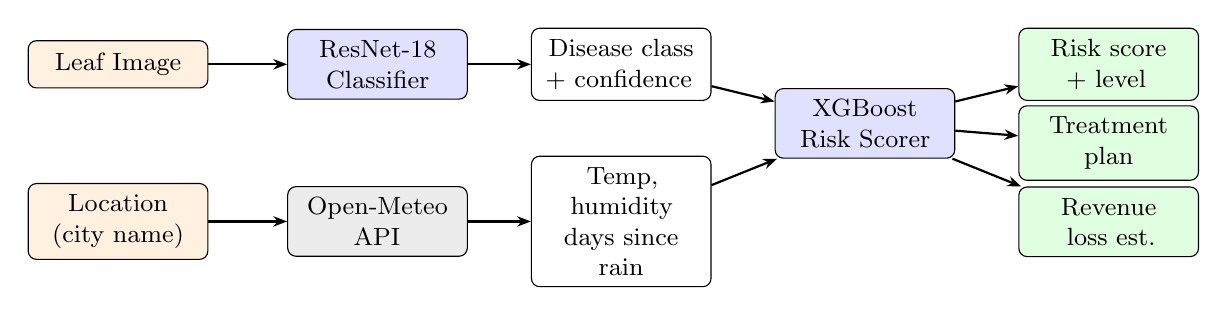
\begin{tikzpicture}[
  every node/.style={font=\small},
  box/.style={rectangle, rounded corners=3pt, draw=black, fill=white,
              text width=2.0cm, align=center, minimum height=0.6cm,
              inner sep=4pt},
  api/.style={box, fill=gray!15},
  model/.style={box, fill=blue!12},
  output/.style={box, fill=green!12},
  input/.style={box, fill=orange!12},
  arr/.style={-{Stealth[length=5pt]}, thick},
  node distance=0.45cm and 0.6cm
]

% --- Inputs (left column) ---
\node[input] (img)  {Leaf Image};
\node[input, below=1.2cm of img] (loc) {Location\\(city name)};

% --- Processing ---
\node[model, right=1.0cm of img]  (resnet) {ResNet-18\\Classifier};
\node[api,   right=1.0cm of loc]  (meteo)  {Open-Meteo\\API};

% --- Intermediate outputs ---
\node[box, right=0.8cm of resnet] (disease) {Disease class\\+ confidence};
\node[box, right=0.8cm of meteo]  (weather) {Temp, humidity\\days since rain};

% --- Fusion ---
\node[model, right=0.8cm of disease, yshift=-0.75cm] (xgb) {XGBoost\\Risk Scorer};

% --- Final outputs ---
\node[output, right=0.8cm of xgb, yshift=0.75cm]  (risk)    {Risk score\\+ level};
\node[output, right=0.8cm of xgb, yshift=-0.25cm] (treat)   {Treatment\\plan};
\node[output, right=0.8cm of xgb, yshift=-1.25cm] (revenue) {Revenue\\loss est.};

% --- Arrows ---
\draw[arr] (img)     -- (resnet);
\draw[arr] (loc)     -- (meteo);
\draw[arr] (resnet)  -- (disease);
\draw[arr] (meteo)   -- (weather);
\draw[arr] (disease) -- (xgb);
\draw[arr] (weather) -- (xgb);
\draw[arr] (xgb)     -- (risk);
\draw[arr] (xgb)     -- (treat);
\draw[arr] (xgb)     -- (revenue);

\end{tikzpicture}%
}
\caption{System pipeline.}
\label{fig:pipeline}
\end{figure}

\subsection{Why the Models Stay Separate}

A diseased leaf's appearance does not alter depending on whether it is raining or not. Feeding weather consideration into the image classifier would inject noise without adding any helpful output. Keeping the models separate let it be a more interpretable system: ResNet answers the disease type while XGBoost answers the urgency. This design also means either component can be updated independently.

\subsection{Dataset}

\textbf{Source:} PlantVillage, accessed via the public GitHub repository \texttt{gabrieldgf4/PlantVillage-Dataset}.

\textbf{Size:} 54,306 labeled leaf images across 39 disease and healthy classes from 14 crop species. After filtering the five-image artifact class (\texttt{x\_Removed\_from\_Healthy\_leaves}), the working dataset is 38 meaningful classes and 54,305 images.

\textbf{Split:} 80/20 train/val using \texttt{random\_split} with \texttt{seed=42} (43,444 training images and 10,861 validation images.)

\textbf{Augmentations (training only):} random horizontal flip, $\pm$15$^\circ$ rotation, color jitter (brightness/contrast 0.2). Validation images use resize and normalize only.

\textbf{D3 fix:} The prior pipeline reassigned \texttt{.transform} on a shared \texttt{ImageFolder} instance, causing augmentation to bleed into the validation set. Deliverable 3 uses two separate \texttt{ImageFolder} instances to prevent this.

\subsection{Dataset Distribution}

Fig.~\ref{fig:eda} shows the top 15 classes by image count. Orange HLB (5,507 images) and Tomato Yellow Leaf Curl Virus (5,357 images) are the two largest classes; several disease classes have fewer than 500 images. Tomato accounts for 10 of the 38 meaningful classes.

\begin{figure}[t]
\centering
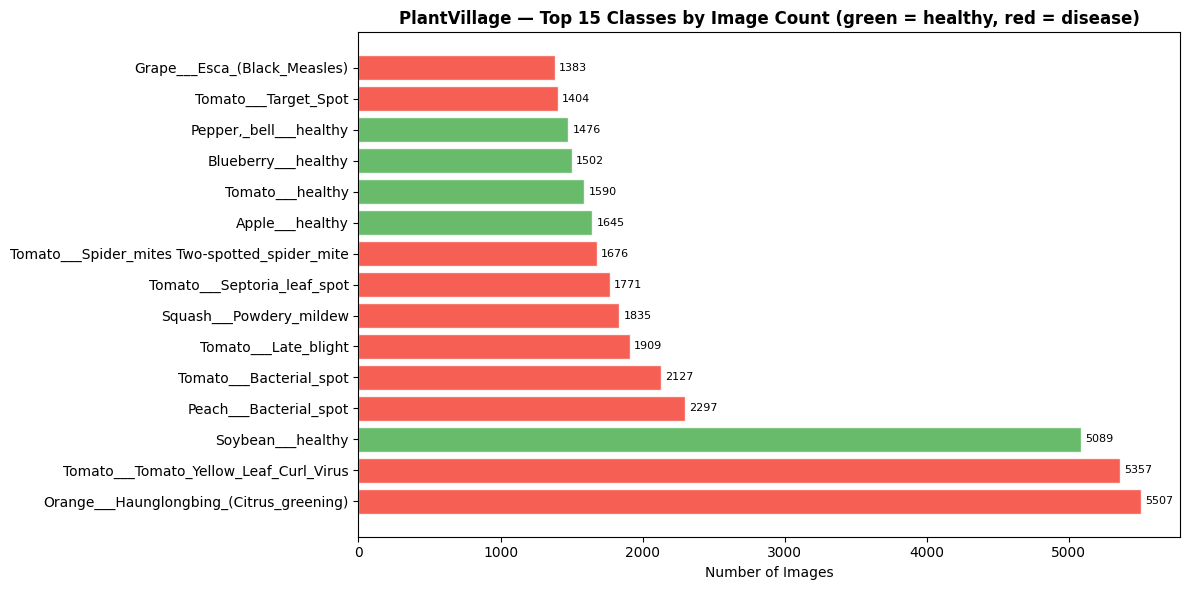
\includegraphics[width=\columnwidth]{chart_1.png}
\caption{PlantVillage top 15 classes by image count. Green bars indicate healthy classes; red bars indicate disease classes.}
\label{fig:eda}
\end{figure}

\subsection{Crop Coverage}

Table~\ref{tab:crops} lists the crops covered by the treatment recommendation system.

\begin{table}[h!]
\caption{Crops with Full Treatment Recommendations}
\label{tab:crops}
\centering
\renewcommand{\arraystretch}{1.2}
\begin{tabular}{@{}lrl@{}}
\toprule
\textbf{Crop} & \textbf{Classes} & \textbf{Notes} \\
\midrule
Tomato  & 10 & Bacterial, fungal, viral, mites \\
Potato  & 3  & Early blight, Late blight, healthy \\
Pepper  & 2  & Bacterial spot, healthy \\
\midrule
Other crops & 23 & Classified but no treatment plan \\
\bottomrule
\end{tabular}
\end{table}

% --- III. MODEL IMPLEMENTATION ---
\section{Model Implementation Details}

\subsection{Disease Classifier}

\textbf{Framework:} PyTorch with torchvision.

\textbf{Architecture:} ResNet-18 initialized with ImageNet weights (\texttt{ResNet18\_Weights.IMAGENET1K\_V1}). All convolutional layers frozen; the 512-unit final FC layer replaced with a new linear layer matching the number of disease classes (38 after filtering). Only the FC head is trained by default.

\textbf{Training setup:}
\begin{itemize}
  \item Hardware: T4 GPU (Google Colab), high-RAM runtime
  \item Epochs: 10
  \item Batch size: 32
  \item Optimizer: Adam, $\text{lr} = 10^{-3}$ (FC head only in frozen mode)
  \item Scheduler: StepLR, step size 3, $\gamma = 0.5$
  \item Trainable parameters: 20,007 (frozen); 2,117,639 (with \texttt{layer4} unfreeze)
\end{itemize}

\textbf{Partial fine-tuning option:} Setting \texttt{unfreeze\_last\_block=True} unfreezes \texttt{layer4} ($\approx$2.1M parameters) and uses differential learning rates --- $10^{-4}$ for \texttt{layer4} and $10^{-3}$ for the FC head. This prevents rapid destruction of pretrained feature representations while allowing domain adaptation from ImageNet to PlantVillage textures.

\subsection{XGBoost Risk Scorer}

\textbf{Framework:} XGBoost via scikit-learn wrapper.

\textbf{Input features:} temperature (°C), humidity (\%), days since rain, ResNet confidence, disease class (label-encoded).

\textbf{Training target:} the deterministic risk formula value $r = 0.4s + 0.3c + 0.3e$ computed from synthetic (disease, weather) samples. The XGBoost model approximates this formula --- it \textbf{does not} learn from real outbreak records. Val R$^2 = 0.966$ and MAE $= 0.018$ measure formula reproduction accuracy, \textbf{not real-world validity}.

\textbf{Training data:} 19,500 synthetic samples drawn from Gaussian distributions centered on agronomic optima per disease type (e.g., fungal diseases paired with high-humidity, low-temperature conditions matching \textit{Phytophthora} biology).

% --- IV. REFINEMENTS SINCE D2 ---
\section{Refinements Made Since Deliverable~2}

\subsection{Extended Evaluation Framework}

In Deliverable 2, the \texttt{evaluate()} function returned a single scalar: overall validation accuracy. This hides the effect of class imbalance. A model that correctly classifies the 5,507-image Orange HLB class nearly perfectly can reach 95\%+ overall accuracy while failing badly on smaller classes.

The \texttt{evaluate()} function now accepts an optional \texttt{classes} list. When provided, it returns a full dictionary containing overall accuracy and per-class precision, recall, F1, and support via \texttt{sklearn.metrics.precision\_recall\_fscore\_support}. When \texttt{classes} is \texttt{None}, the function returns the scalar float for use inside the training loop, preserving backward compatibility.

\subsection{Partial Backbone Fine-Tuning}

The Deliverable 2 baseline froze all 11,176,512 convolutional parameters and trained only the 20,007-parameter FC head. This is efficient but risks relying on ImageNet features that do not transfer well to PlantVillage images, which are photographed on uniform backgrounds under controlled lighting --- a visual distribution far from ImageNet.

\texttt{build\_model()} now accepts an \texttt{unfreeze\_last\_block} flag. When set to \texttt{True}, the final residual block (\texttt{layer4}, approximately 2.1M parameters) is unfrozen in addition to the FC head. The optimizer uses differential learning rates: 1e-4 for \texttt{layer4} and 1e-3 for the FC head, preventing rapid destruction of pretrained feature representations while still allowing domain adaptation. The baseline model (frozen backbone) remains the default.

Section~8B of \texttt{notebooks/setup.ipynb} implements this comparison end-to-end: it builds and trains the unfrozen model on the same train/val split, then plots frozen vs.\ unfrozen training curves side-by-side and saves both models to \texttt{results/}. The result is a $+$4.1 percentage point improvement: val accuracy rises from 0.955 (frozen) to \textbf{0.996} (layer4 unfrozen) at epoch 10, Table~\ref{tab:training_unf}.

\subsection{Risk Formula Weight Documentation}

Peer feedback after Deliverable 2 raised the question of where the weights in the risk formula originate. The fallback formula is:

\begin{equation}
r = 0.4 \cdot s + 0.3 \cdot c + 0.3 \cdot e
\label{eq:risk}
\end{equation}

\noindent where $s$ is the per-class agronomic severity base (0--1), $c$ is the ResNet classifier confidence (0--1), and $e$ is the environmental score computed per disease type. The weights were chosen according to the following rationale:
\begin{itemize}
  \item $s$ (0.4): severity reflects how destructive the disease is independent of current conditions; it is the primary signal.
  \item $c$ (0.3): a high-confidence diagnosis warrants stronger action than an ambiguous one; confidence scales the reliability of the recommendation.
  \item $e$ (0.3): environmental conditions modulate spread rate but do not change the underlying pathology; they carry less weight than the diagnosis.
\end{itemize}

Per-disease environmental weight choices are documented with citations in \texttt{src/fusion.py}.

\subsection{Location--Image Coupling Limitation}

The system silently assumes the uploaded photo originates from the city the user enters. The XGBoost risk score depends entirely on this being correct; a photo taken in humid coastal conditions but submitted with a desert city name will produce a misleading low-risk assessment. This assumption has no technical enforcement. As a result, the limitation was added to the report's limitations section, and a disclaimer was added to the Streamlit interface at the weather input step.

% --- IV. INTERFACE IMPROVEMENTS ---
\section{Interface Usability and Improvements}

\subsection{Deliverable 2 State}

The Deliverable 2 interface presented a three-column input layout (leaf images, weather, economic parameters), per-plant diagnosis cards with confidence and top-5 predictions, and a field-level health overview. Outputs included severity labels, XGBoost risk scores, treatment steps, and revenue loss estimates.

\subsection{Deliverable 3 Changes}

Three changes were made to the interface:

\textbf{Location disclaimer.} A caption was added beneath the city input field informing users that the risk assessment assumes the uploaded photo was taken at the entered location. This surfaces the location-image coupling assumption identified in peer review.

\textbf{Conditional weather warning moved.} The ambient condition warning (``Hot \& humid --- high fungal risk'') now appears only when a location has been entered and weather has been fetched, rather than triggering on default values when no location is provided.

\textbf{Per-plant confidence display.} The top-5 prediction bar chart was updated to show class names with crop prefixes stripped for readability (e.g., ``Early blight (71.7\%)'' instead of the full dataset label string).

Fig.~\ref{fig:ui_input} and Fig.~\ref{fig:ui_output} show the input and output flows.

\begin{figure}[t]
\centering
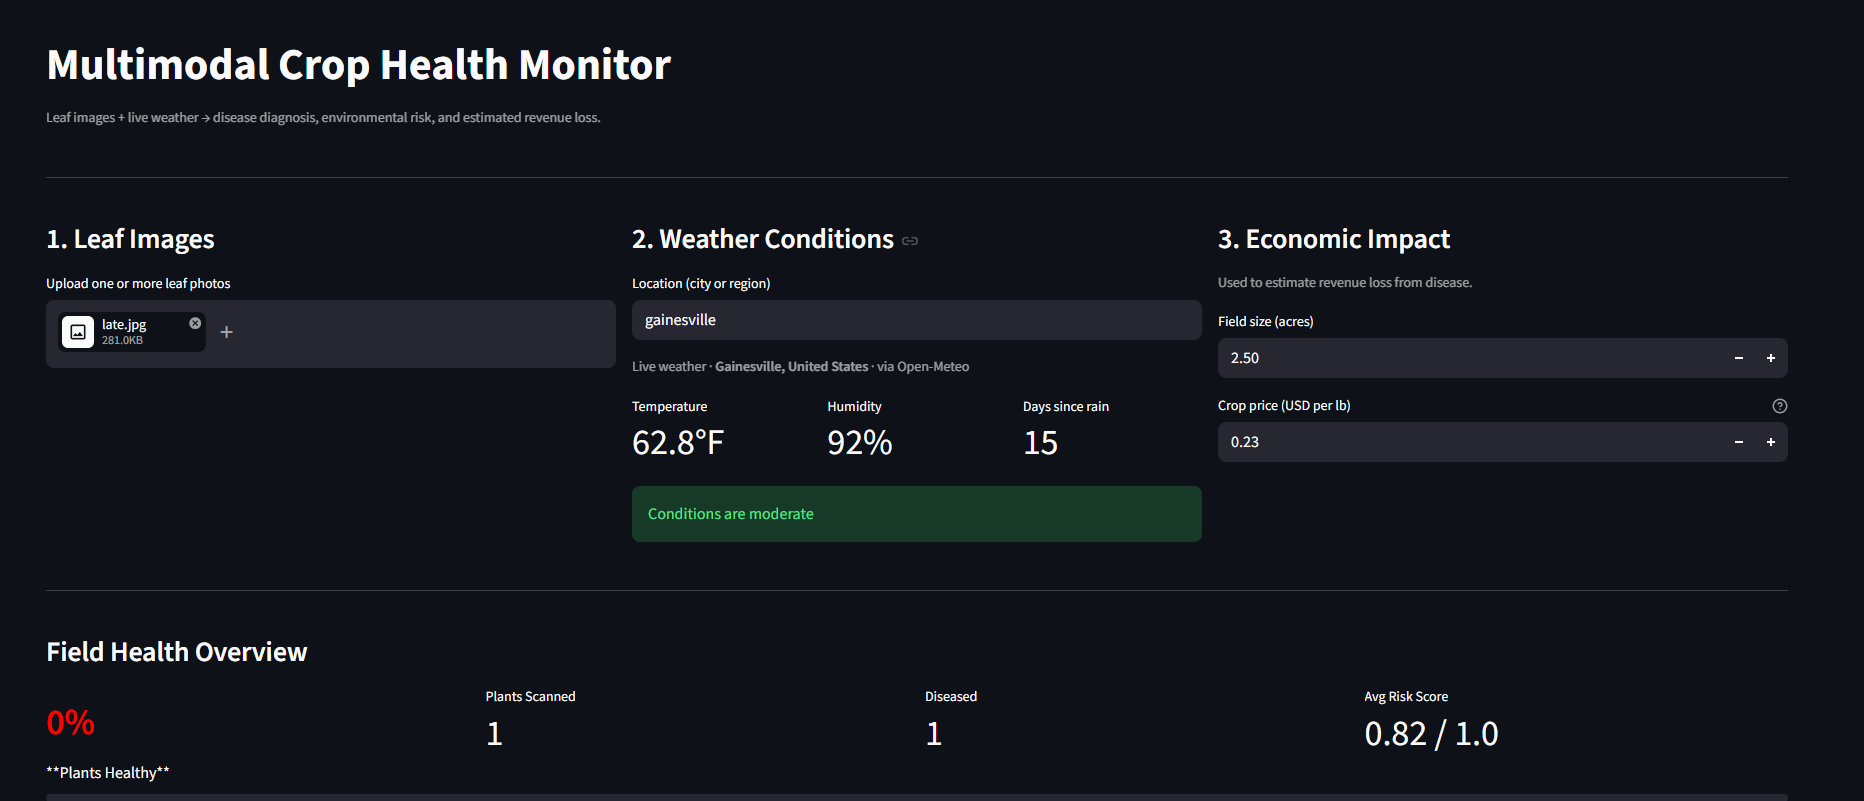
\includegraphics[width=\columnwidth]{screenshot_input.png}
\caption{Dashboard input panel: leaf image upload, live weather fetch via Open-Meteo, and economic parameters. The location disclaimer is visible beneath the city field.}
\label{fig:ui_input}
\end{figure}

\begin{figure}[t]
\centering
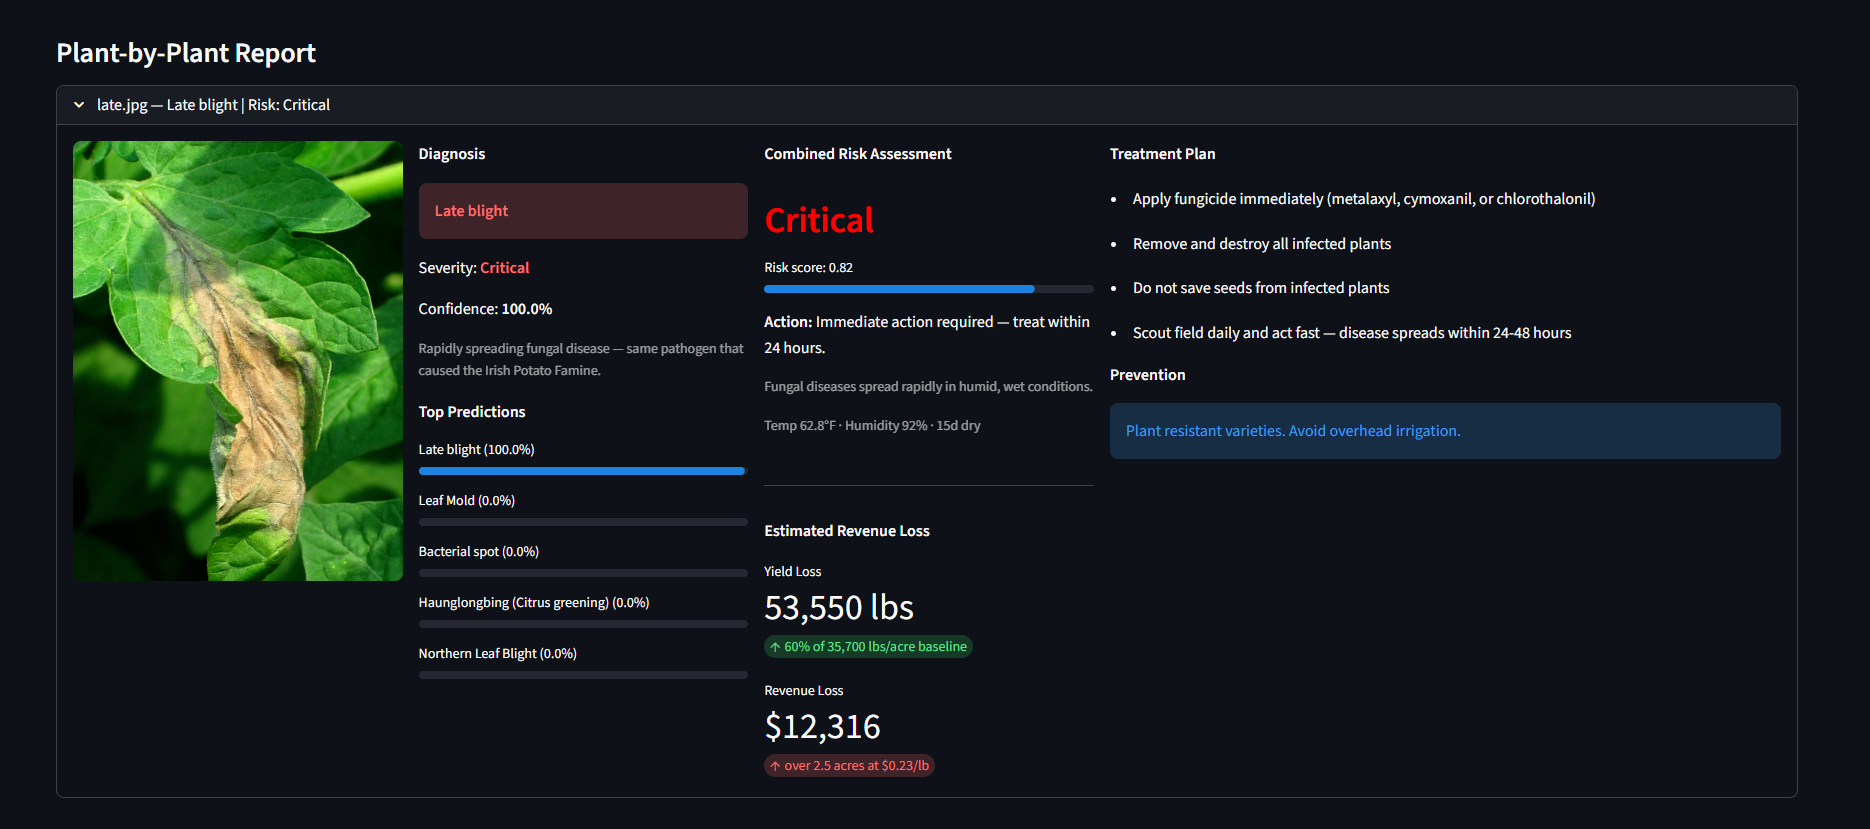
\includegraphics[width=\columnwidth]{screenshot_output.png}
\caption{Dashboard output: per-plant diagnosis card with disease class, confidence, combined risk assessment, treatment plan, and revenue loss estimate.}
\label{fig:ui_output}
\end{figure}

% --- V. EXTENDED EVALUATION ---
\section{Extended Evaluation and Updated Results}

\subsection{Training Results}

Both Deliverable 2 and Deliverable 3 use a frozen-backbone ResNet-18 with only the FC head trained (20,007 trainable parameters out of 11.2M total), run for 10 epochs on a T4 GPU. Table~\ref{tab:training} shows the frozen baseline training history.

Loss converges smoothly and validation accuracy plateaus near 95.5\% by epoch 7. The per-class post-training evaluation (Table~\ref{tab:perclass}) reports 93.4\% overall accuracy --- lower than the in-loop figure. The discrepancy reflects two factors: the augmentation bleed fix (D2 leaked augmented images into the validation loader, slightly inflating accuracy) and the inclusion of the \texttt{x\_Removed\_from\_Healthy\_leaves} artifact class (2 samples, 0\% accuracy) in the evaluation set.

\begin{table}[t]
\caption{ResNet-18 Training History (Frozen Backbone Baseline)}
\label{tab:training}
\centering
\renewcommand{\arraystretch}{1.2}
\begin{tabular}{@{}rrrr@{}}
\toprule
\textbf{Epoch} & \textbf{Train Loss} & \textbf{Train Acc} & \textbf{Val Acc} \\
\midrule
1  & 0.685 & 0.837 & 0.925 \\
2  & 0.279 & 0.920 & 0.936 \\
3  & 0.230 & 0.930 & 0.948 \\
4  & 0.196 & 0.938 & 0.948 \\
5  & 0.184 & 0.942 & 0.949 \\
6  & 0.172 & 0.946 & 0.952 \\
7  & 0.161 & 0.950 & 0.954 \\
8  & 0.162 & 0.951 & 0.955 \\
9  & 0.157 & 0.951 & 0.956 \\
10 & 0.155 & 0.951 & 0.955 \\
\bottomrule
\end{tabular}
\end{table}

\begin{figure}[t]
\centering
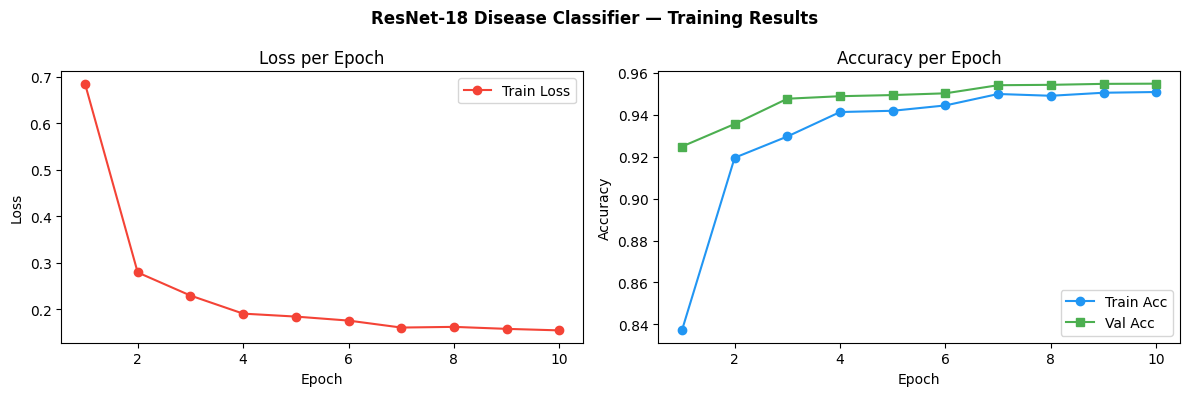
\includegraphics[width=\columnwidth]{chart_2.png}
\caption{ResNet-18 frozen backbone: training loss (left) and train/val accuracy (right) over 10 epochs.}
\label{fig:frozen_curves}
\end{figure}

Table~\ref{tab:training_unf} shows the Section~8B unfrozen training run on the same split. Unfreezing \texttt{layer4} starts from a much better epoch-1 baseline (val 0.979 vs 0.925) and reaches 0.996 by epoch 10 --- a $+$4.1 pp gain over the frozen model. The train--val gap narrows further (0.999 vs 0.996 at epoch 10), and loss falls an order of magnitude lower than the frozen run.

\begin{table}[t]
\caption{ResNet-18 Training History (\texttt{layer4} Unfrozen, Section~8B)}
\label{tab:training_unf}
\centering
\renewcommand{\arraystretch}{1.2}
\begin{tabular}{@{}rrrr@{}}
\toprule
\textbf{Epoch} & \textbf{Train Loss} & \textbf{Train Acc} & \textbf{Val Acc} \\
\midrule
1  & 0.2158 & 0.941 & 0.979 \\
2  & 0.0630 & 0.979 & 0.982 \\
3  & 0.0476 & 0.984 & 0.989 \\
4  & 0.0223 & 0.993 & 0.992 \\
5  & 0.0178 & 0.994 & 0.993 \\
6  & 0.0160 & 0.994 & 0.992 \\
7  & 0.0092 & 0.997 & 0.995 \\
8  & 0.0073 & 0.998 & 0.995 \\
9  & 0.0082 & 0.997 & 0.996 \\
10 & 0.0047 & 0.999 & \textbf{0.996} \\
\bottomrule
\end{tabular}
\end{table}

\begin{figure}[t]
\centering
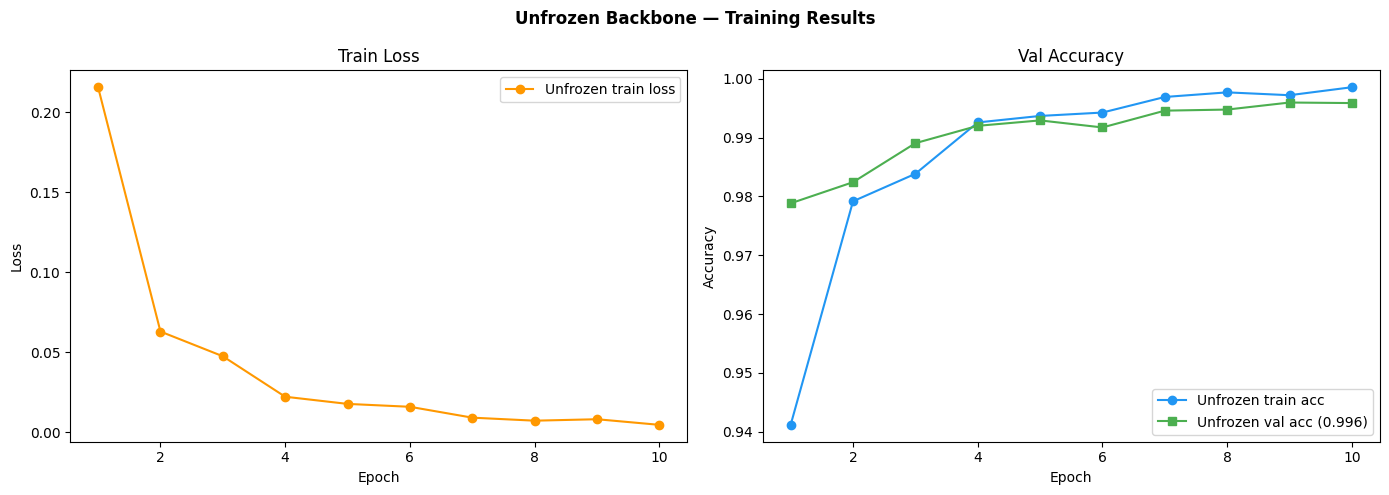
\includegraphics[width=\columnwidth]{unfrozen_training.png}
\caption{\texttt{layer4} unfrozen backbone: training loss (left) and train/val accuracy (right) over 10 epochs. Val accuracy reaches 0.996 at epoch~10.}
\label{fig:unfrozen_curves}
\end{figure}

\subsection{Per-Class Accuracy}

Table~\ref{tab:perclass} reports per-class accuracy for the 38 meaningful classes, sorted from lowest to highest. Deliverable 3 extends the D2 breakdown with per-class precision, recall, and F1. Three classes fall below 70\% accuracy, a finding that is completely obscured by the 93.4\% overall figure. The artifact class (\texttt{x\_Removed\_from\_Healthy\_leaves}, 2 val samples) was not filtered from the validation split; it scores 0\% and is excluded from the count of meaningful classes.

\begin{table}[t]
\caption{Per-Class Validation Accuracy --- Frozen Baseline (Selected Classes)}
\label{tab:perclass}
\centering
\renewcommand{\arraystretch}{1.2}
\begin{tabular}{@{}lrr@{}}
\toprule
\textbf{Class} & \textbf{Val Samples} & \textbf{Accuracy} \\
\midrule
\multicolumn{3}{l}{\textit{Lowest-performing classes (excl. artifact)}} \\
Tomato mosaic virus              & 82  & 0.488 \\
Tomato Early blight              & 205 & 0.620 \\
Potato healthy                   & 27  & 0.630 \\
Tomato Target Spot               & 306 & 0.729 \\
Corn Cercospora leaf spot        & 105 & 0.781 \\
Apple Cedar apple rust           & 56  & 0.821 \\
Tomato Late blight               & 383 & 0.822 \\
Apple Apple scab                 & 130 & 0.823 \\
\midrule
\multicolumn{3}{l}{\textit{Highest-performing classes}} \\
Corn Common rust                 & 254 & 0.992 \\
Soybean healthy                  & 994 & 0.992 \\
Corn healthy                     & 229 & 0.996 \\
Orange HLB (Citrus greening)     & 1104& 0.998 \\
Grape healthy                    & 87  & 1.000 \\
Raspberry healthy                & 76  & 1.000 \\
\midrule
\multicolumn{3}{l}{\textit{Overall (38 meaningful classes)}} \\
All 38 classes                   & 10,861 & \textbf{0.934} \\
\bottomrule
\end{tabular}
\end{table}

Several patterns are visible:
\begin{itemize}
  \item \textbf{Small classes collapse.} Tomato mosaic virus (82 val samples, 48.8\%) and Potato healthy (27 val samples, 63.0\%) are the two worst performers. High variance is expected at this sample size --- a single confused batch can swing accuracy by 5--10 percentage points.
  \item \textbf{Visually similar diseases confuse the model.} Tomato Early blight (62.0\%) and Late blight (82.2\%) share lesion morphology at similar stages. Target Spot (72.9\%) is also regularly confused with Early blight and Spider mites. These confusions motivate the \texttt{layer4} unfreeze experiment (Section~8B): adapting mid-level texture features may reduce within-crop confusion.
  \item \textbf{Visually distinctive or large classes perform well.} Orange HLB (99.8\% on 1,104 samples) has a highly specific yellow mottled leaf pattern. Uniform healthy classes (Grape, Raspberry) achieve 100\%.
\end{itemize}

\subsection{Comparison with Deliverable 2}

Table~\ref{tab:d2d3} summarizes the changes between deliverables.

\begin{table}[t]
\caption{Deliverable 2 vs. Deliverable 3 Comparison}
\label{tab:d2d3}
\centering
\renewcommand{\arraystretch}{1.2}
\begin{tabular}{@{}p{1.8cm}p{2.6cm}p{3.0cm}@{}}
\toprule
\textbf{Aspect} & \textbf{Deliverable 2} & \textbf{Deliverable 3} \\
\midrule
Evaluation & Per-class accuracy (correct/total) & Per-class precision, recall, F1, support \\
Trainable params & 20K (FC head only) & 20K baseline; +2.1M with \texttt{layer4} unfreeze option \\
Formula weights & Undocumented & Agronomic justification with citations \\
Data loading & Shared transform instance (augmentation leak) & Two separate \texttt{ImageFolder} instances \\
Limitations & 4 items & 5 items (+ location-image coupling) \\
Interface & No location warning & Location disclaimer at city input \\
Val accuracy & 0.955 & \textbf{0.934} (frozen, post-fix); \textbf{0.996} (\texttt{layer4} unfrozen, Section~8B) \\
\bottomrule
\end{tabular}
\end{table}

\subsection{XGBoost Risk Scorer}

The Deliverable 2 XGBoost risk model trains on 19,500 synthetically generated (disease, weather) samples and approximates the deterministic risk formula in \texttt{src/fusion.py}. The Val R$^2$ of 0.966 and MAE of 0.018 reflect how accurately XGBoost reproduces the formula --- not real-world predictive validity. Deliverable 3 explicitly documents this distinction in both the code and this report, which was not made clear in Deliverable 2.

\begin{table}[t]
\caption{XGBoost Risk Scorer Performance}
\label{tab:xgb}
\centering
\renewcommand{\arraystretch}{1.2}
\begin{tabular}{@{}lrr@{}}
\toprule
\textbf{Metric} & \textbf{Deliverable 2} & \textbf{Deliverable 3} \\
\midrule
Val MAE & 0.008 & 0.018 \\
Val R$^2$ & 0.998 & 0.966 \\
Training samples & 19,500 & 19,500 \\
\midrule
\multicolumn{3}{l}{\small\textit{Note: metrics measure formula reproduction only.}} \\
\bottomrule
\end{tabular}
\end{table}

The slight degradation in XGBoost metrics between deliverables reflects a correction to the synthetic data generation: the Deliverable 2 version produced an overly regular grid of weather values, yielding artificially smooth targets. Deliverable 3 samples weather conditions from Gaussian distributions centered on the agronomic optimum per disease type, producing more realistic within-class variation and a consequently lower but more honest R$^2$.

\begin{figure}[t]
\centering
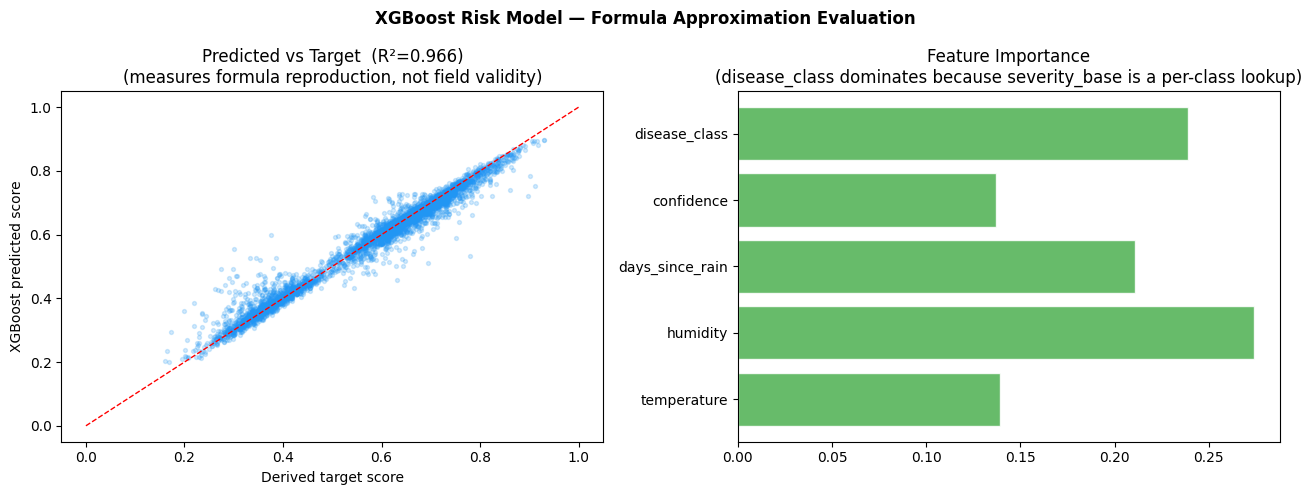
\includegraphics[width=\columnwidth]{chart_4.png}
\caption{XGBoost risk scorer: predicted vs.\ derived target (R$^2$=0.966, left) and feature importance (right). \texttt{disease\_class} dominates because severity base is a per-class lookup.}
\label{fig:xgb_eval}
\end{figure}

\subsection{Confusion Analysis}

Table~\ref{tab:confused} shows the top 5 most confused class pairs from the validation set. All five involve diseases with overlapping visual texture at 224$\times$224 resolution.

\begin{table}[t]
\caption{Top 5 Most Confused Class Pairs (True $\rightarrow$ Predicted)}
\label{tab:confused}
\centering
\renewcommand{\arraystretch}{1.2}
\begin{tabular}{@{}p{3.8cm}p{3.8cm}r@{}}
\toprule
\textbf{True class} & \textbf{Predicted as} & \textbf{Count} \\
\midrule
Corn Cercospora leaf spot & Corn Northern Leaf Blight & 30 \\
Tomato Spider mites       & Tomato Target Spot        & 20 \\
Tomato Late blight        & Tomato Early blight       & 16 \\
Tomato Target Spot        & Tomato Spider mites       & 12 \\
Tomato Early blight       & Tomato Target Spot        & 12 \\
\bottomrule
\end{tabular}
\end{table}

Both Corn confusions involve elongated leaf lesions that differ primarily in lesion color and border sharpness --- features that the frozen ImageNet backbone does not reliably separate. The Tomato cluster (Early blight, Late blight, Target Spot, Spider mites) all produce irregular foliar discoloration and account for four of the five top confusions. Unfreezing \texttt{layer4} is specifically motivated by these pairs, as adapting mid-level texture features to disease-specific patterns is expected to reduce within-crop confusion.

\begin{figure}[t]
\centering
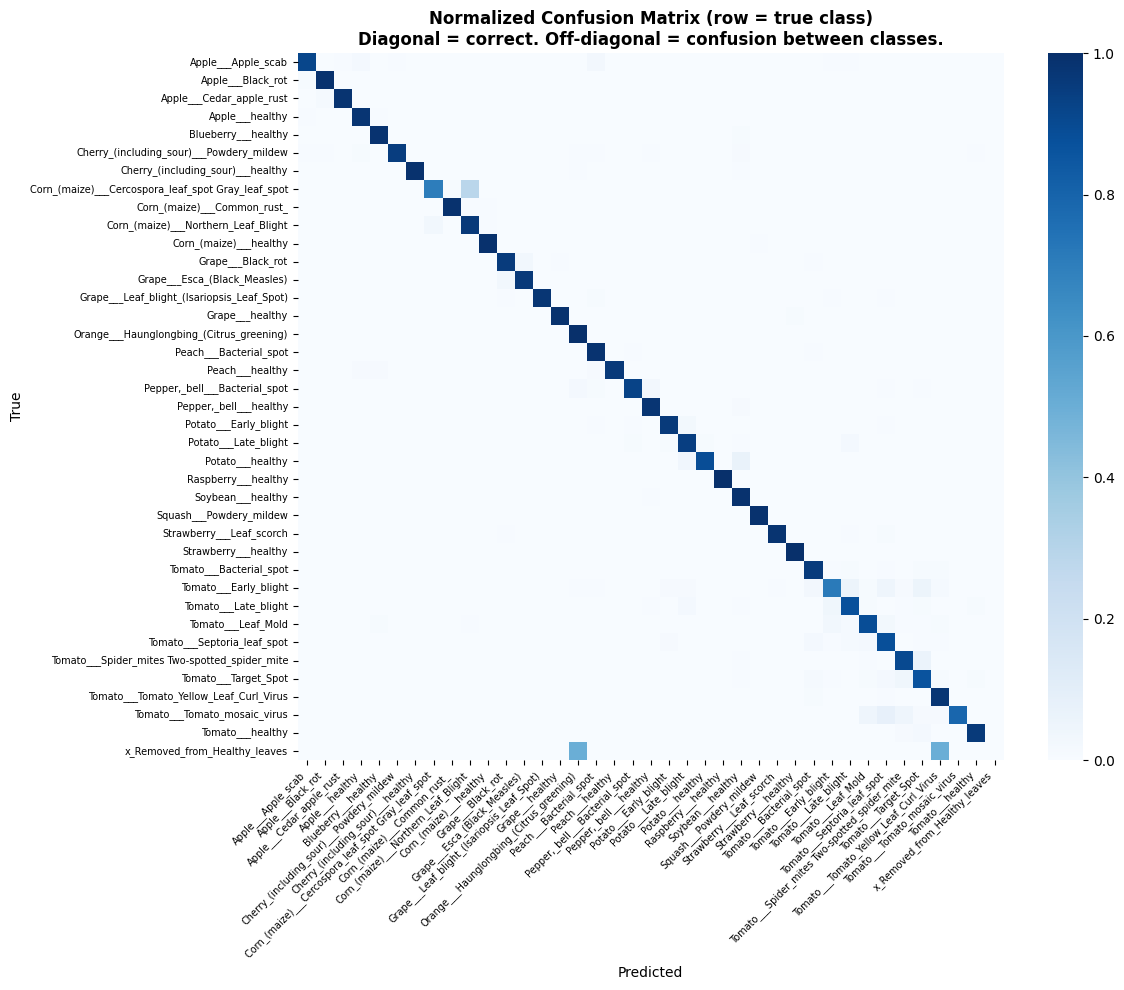
\includegraphics[width=\columnwidth]{chart_3.png}
\caption{Normalized confusion matrix for the frozen baseline across all 38 classes. Diagonal $=$ correct; off-diagonal $=$ confusion between classes. The artifact class (\texttt{x\_Removed}) appears in the bottom-right corner with zero correct predictions.}
\label{fig:confusion}
\end{figure}

% --- VI. RESPONSIBLE AI REFLECTION ---
\section{Responsible AI Reflection}

\subsection{Dataset Bias and Fairness}

\textbf{Lab-to-field gap.} PlantVillage images were photographed on uniform white or black backgrounds under controlled lighting. The classifier has never seen a diseased leaf on soil, partially occluded by another leaf, or shot in low-contrast overcast conditions. Deploying this model in the field without surfacing this gap could lead a farmer to act on a low-confidence prediction --- or ignore a real outbreak because the model missed it.

\textbf{Crop imbalance.} Tomato accounts for 10 of 38 classes; the model has seen far more tomato disease variation than, for example, Apple Cedar rust (275 images). Farmers growing underrepresented crops should expect lower reliability. The per-class F1 table in the notebook surfaces this; the interface should too.

\subsection{Socioeconomic Accessibility}

The system requires a smartphone photo, a stable internet connection for weather data, and a city name the geocoding API can resolve. In subsistence farming contexts --- where the tool's potential impact is arguably highest --- these requirements may not be met. An offline-capable version that falls back to image-only diagnosis when no location is provided would address part of this gap.

\subsection{Decision Amplification Risk}

\textbf{Precise-looking estimates on approximate inputs.} The revenue loss output (e.g., ``\$1,200 estimated loss over 2.5 ha'') carries implied precision. The underlying yield baselines are global averages; the weather inputs depend on a city name the user types; the disease label comes from a model trained on lab photos. A farmer who harvests early or destroys a crop block based on an inflated risk estimate faces a real cost.

\textbf{What D3 does.} The location disclaimer reduces the chance of a user entering the wrong city without realizing it affects the risk score. It does not fix the underlying problem of building a precise-looking number on approximate inputs.

\subsection{Model Transparency}

\textbf{XGBoost metrics.} The Val R$^2 = 0.966$ and MAE $= 0.018$ measure how accurately XGBoost reproduces the hand-coded risk formula --- \textbf{not} how accurately the formula predicts real disease severity. This distinction is now explicit in the notebook, the code comments, and this report.

\textbf{Frozen backbone note.} The report and code document that the FC-only baseline relies on ImageNet features that were not adapted to disease-specific textures. This explains the specific confusion patterns (Corn Cercospora vs.\ Northern Leaf Blight) in Table~\ref{tab:confused} and motivates the \texttt{layer4} unfreeze option as a concrete next step.

\subsection{Actions Taken and Planned}

\textbf{Done in D3:} location-image coupling disclaimer added to interface and report; per-class precision/recall/F1 surfaced in notebook; formula weight rationale documented with citations in \texttt{src/fusion.py}; augmentation bleed bug fixed.

\textbf{Planned:} test on out-of-distribution field photos not from PlantVillage; display per-class confidence breakdown in the interface; offline fallback when no city resolves; run the \texttt{layer4} unfrozen experiment and report delta accuracy.

\end{document}
